\documentclass{standalone}
\usepackage{picture,color}
\usepackage{graphicx}
\graphicspath{{./scan_1_raw/}}
\setlength{\unitlength}{1in}
\renewcommand{\rmdefault}{phv} % Arial
\renewcommand{\sfdefault}{phv} % Arial

\begin{document}
\begin{picture}(7.8, 2.53)(.12, -2.651)
% \put(0.15, -.65){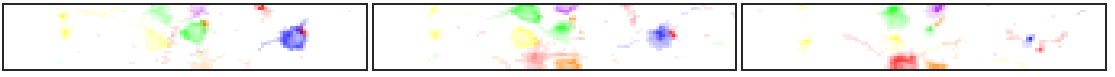
\includegraphics[height=0.49in]{spatial_overlap_1_10_1.pdf}}
% \put(0.15, -1.15){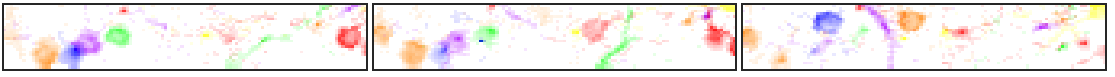
\includegraphics[height=0.49in]{spatial_overlap_11_30_1.pdf}}
% \put(0.15, -1.65){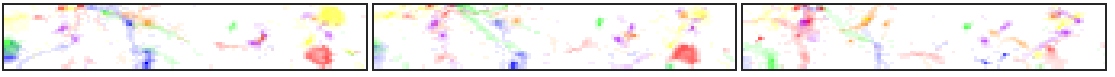
\includegraphics[height=0.49in]{spatial_overlap_31_60_1.pdf}}
% \put(0.15, -2.15){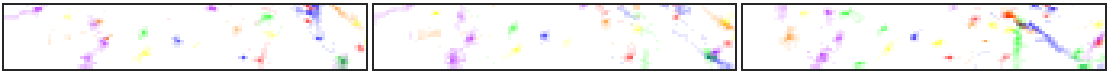
\includegraphics[height=0.49in]{spatial_overlap_61_100_1.pdf}}
% \put(0.15, -2.65){\includegraphics[height=0.49in]{spatial_overlap_101_Inf_1.pdf}}
\put(0.29, -.65){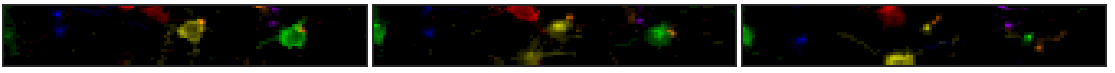
\includegraphics[height=0.49in]{spatial_overlap_1_10_0.pdf}}
\put(0.29, -1.15){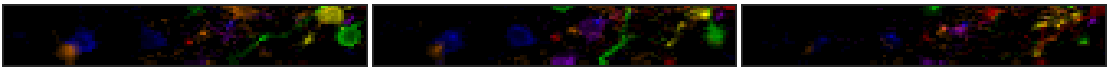
\includegraphics[height=0.49in]{spatial_overlap_11_30_0.pdf}}
\put(0.29, -1.65){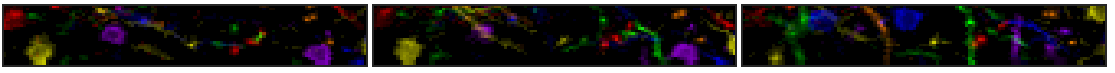
\includegraphics[height=0.49in]{spatial_overlap_31_60_0.pdf}}
\put(0.29, -2.15){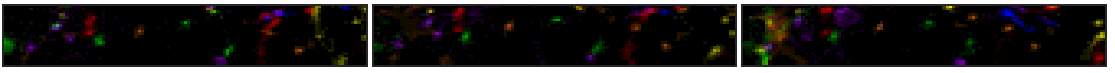
\includegraphics[height=0.49in]{spatial_overlap_61_100_0.pdf}}
\put(0.29, -2.65){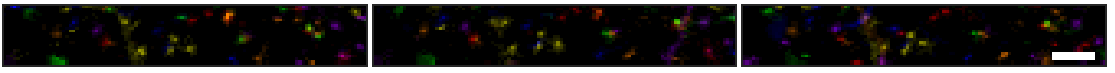
\includegraphics[height=0.49in]{spatial_overlap_101_Inf_0.pdf}}
\multiput(0.14, -0.625)(0, 0.46){2}{\color{black}\line(1, 0){7.75}}
\multiput(0.14, -0.625)(7.75,0){2}{\color{black}\line(0, 1){0.46}}

\multiput(0.14, -1.125)(0, 0.46){2}{\color{black}\line(1, 0){7.75}}
\multiput(0.14, -1.125)(7.75,0){2}{\color{black}\line(0, 1){0.46}}

\multiput(0.14, -1.625)(0, 0.46){2}{\color{black}\line(1, 0){7.75}}
\multiput(0.14, -1.625)(7.75,0){2}{\color{black}\line(0, 1){0.46}}

\multiput(0.14, -2.125)(0, 0.46){2}{\color{black}\line(1, 0){7.75}}
\multiput(0.14, -2.125)(7.75,0){2}{\color{black}\line(0, 1){0.46}}

\multiput(0.14, -2.625)(0, 0.46){2}{\color{black}\line(1, 0){7.75}}
\multiput(0.14, -2.625)(7.75,0){2}{\color{black}\line(0, 1){0.46}}
\end{picture}
\end{document}\grid
